% Copyright 2021  Ed Bueler

\documentclass[xcolor={svgnames},
               hyperref={colorlinks,citecolor=DeepPink4,linkcolor=FireBrick,urlcolor=Maroon}]
               {beamer}

\mode<presentation>{
  \usetheme{Madrid}
  \usecolortheme{seagull}
  \setbeamercovered{transparent}
  \setbeamerfont{frametitle}{size=\large}
}

\setbeamercolor*{block title}{bg=red!10}
\setbeamercolor*{block body}{bg=red!5}

\usepackage[english]{babel}
\usepackage[latin1]{inputenc}
\usepackage{times}
\usepackage[T1]{fontenc}
% Or whatever. Note that the encoding and the font should match. If T1
% does not look nice, try deleting the line with the fontenc.

\usepackage{empheq,bm}
\usepackage{xspace}
\usepackage{fancyvrb}

\usepackage{tikz}
\usetikzlibrary{shapes,arrows.meta,decorations.markings,decorations.pathreplacing,fadings,positioning}

\usepackage[kw]{pseudo}
\pseudoset{left-margin=15mm,topsep=5mm,idfont=\texttt,st-left=,st-right=}


% If you wish to uncover everything in a step-wise fashion, uncomment
% the following command:
%\beamerdefaultoverlayspecification{<+->}

\newcommand{\ba}{\mathbf{a}}
\newcommand{\bb}{\mathbf{b}}
\newcommand{\bc}{\mathbf{c}}
\newcommand{\bbf}{\mathbf{f}}
\newcommand{\bg}{\mathbf{g}}
\newcommand{\bn}{\mathbf{n}}
\newcommand{\bq}{\mathbf{q}}
\newcommand{\br}{\mathbf{r}}
\newcommand{\bx}{\mathbf{x}}
\newcommand{\by}{\mathbf{y}}
\newcommand{\bv}{\mathbf{v}}
\newcommand{\bu}{\mathbf{u}}
\newcommand{\bw}{\mathbf{w}}

\newcommand{\bF}{\mathbf{F}}
\newcommand{\bG}{\mathbf{G}}
\newcommand{\bQ}{\mathbf{Q}}

\newcommand{\grad}{\nabla}
\newcommand{\Div}{\nabla\cdot}
\newcommand{\minmod}{\operatorname{minmod}}

\newcommand{\CC}{\mathbb{C}}
\newcommand{\RR}{\mathbb{R}}

\newcommand{\ddt}[1]{\ensuremath{\frac{\partial #1}{\partial t}}}
\newcommand{\ddx}[1]{\ensuremath{\frac{\partial #1}{\partial x}}}
\newcommand{\Matlab}{\textsc{Matlab}\xspace}
\newcommand{\Octave}{\textsc{Octave}\xspace}
\newcommand{\eps}{\epsilon}

\newcommand{\ip}[2]{\left<#1,#2\right>}

\newcommand{\xiphalf}{{x_{i+\frac{1}{2}}}}
\newcommand{\ximhalf}{{x_{i-\frac{1}{2}}}}
\newcommand{\Fiphalf}{{F_{i+\frac{1}{2}}}}
\newcommand{\Fimhalf}{{F_{i-\frac{1}{2}}}}
\newcommand{\Fiphalfn}{{F^n_{i+\frac{1}{2}}}}
\newcommand{\Fimhalfn}{{F^n_{i-\frac{1}{2}}}}

\newcommand{\trefcolumn}[1]{\begin{bmatrix} \phantom{x} \\ #1 \\ \phantom{x} \end{bmatrix}}
\newcommand{\trefmatrixtwo}[2]{\left[\begin{array}{c|c|c} & & \\ #1 & \dots & #2 \\ & & \end{array}\right]}
\newcommand{\trefmatrixthree}[3]{\left[\begin{array}{c|c|c|c} & & & \\ #1 & #2 & \dots & #3 \\ & & & \end{array}\right]}
\newcommand{\trefmatrixgroups}[4]{\left[\begin{array}{c|c|c|c|c|c} & & & & & \\ #1 & \dots & #2 & #3 & \dots & #4 \\ & & & & & \end{array}\right]}

\newcommand{\blocktwo}[4]{\left[\begin{array}{c|c} #1 & #2 \\ \hline #3 & #4 \end{array}\right]}

\newcommand{\bqed}{{\color{blue}\qed}}
\newcommand{\ds}{\displaystyle}

\newcommand\mynum[1]{{\renewcommand{\insertenumlabel}{#1}%
      \usebeamertemplate{enumerate item} \,}}


\title{Online optimization}

\subtitle{\emph{what's the goal of ML training algorithms? minimize regret!}}

\author{Ed Bueler}

\institute[UAF]{MATH 692 Mathematics for Machine Learning \\ UAF}

\date[Spring 2022]{17 March}

%\titlegraphic{\begin{picture}(0,0)
%    \put(0,180){\makebox(0,0)[rt]{\includegraphics[width=4cm]{figs/software.png}}}
%  \end{picture}
%}

%% this nonsense needed to start section counter at 0; see
%% https://tex.stackexchange.com/questions/170222/change-the-numbering-in-beamers-table-of-content
\makeatletter
\patchcmd{\beamer@sectionintoc}
  {\ifnum\beamer@tempcount>0}
  {\ifnum\beamer@tempcount>-1}
  {}
  {}
%\beamer@tocsectionnumber=-1
\makeatother


\begin{document}
\beamertemplatenavigationsymbolsempty

\begin{frame}
  \maketitle
\end{frame}



\begin{frame}{today's talk}

\begin{itemize}
\item fixme

\begin{center}
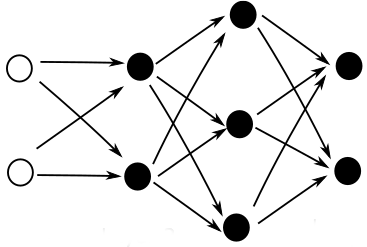
\includegraphics[height=30mm]{figs/cleannet.png}
\end{center}

\end{itemize}
\end{frame}


\begin{frame}{references}

\begin{itemize}
\footnotesize
\item I.~Goodfellow, Y.~Bengio, \& A.~Courville, \href{https://www.deeplearningbook.org/}{\emph{Deep Learning.}} MIT Press, 2016
    \begin{itemize}
    \scriptsize
    \item[$-$] Chapter 8 addresses empirical risk, but online optimization is not mentioned
    \end{itemize}
\item D.~P.~Kingma \& J.~Ba (2014). \href{https://arxiv.org/abs/1412.6980}{\emph{Adam: A method for stochastic optimization.}}, arXiv preprint arXiv:1412.6980.
    \begin{itemize}
    \scriptsize
    \item[$-$] 100651 citations
    \item[$-$] cites Zinkevich (2003) for online optimization framework
    \end{itemize}
\item M.~Zinkevich (2003). \href{https://www.aaai.org/Papers/ICML/2003/ICML03-120.pdf}{\emph{Online convex programming and generalized infinitesimal gradient ascent.}} Proceedings of the 20th International Conference on Machine Learning, 928-936
%\item C.~F.~Higham \& D.~J.~Higham (2019). \href{http://www.math.stonybrook.edu/~bishop/classes/math533.S21/MachineLearning/SIAMreview.pdf}{\emph{Deep learning: An introduction for applied mathematicians.}} SIAM Review, 61(4), 860-891
\end{itemize}
\end{frame}






\end{document}
